% Canary Signal Flow — RayaChain (OMN-175)
% UML-style swimlane activity diagram
% 4 lanes: Miner · Validator · Canary Layer · Consumer
% 5 activities; OMN-176 insertion hook at A3 (validator scoring)
% Compile: pdflatex canary-signal-flow.tex
%
% Tight-page trick: \pdfpagewidth/height set to bounding box of figbox.
\documentclass{article}
\usepackage[margin=0pt]{geometry}
\pagestyle{empty}
\usepackage[T1]{fontenc}
\usepackage{lmodern}
\usepackage{tikz}
\usetikzlibrary{arrows.meta,backgrounds}

%% ---- Palette (matches OmniRisk five-engine diagram) ----------------
\definecolor{minerfill}{HTML}{f0fdf4}
\definecolor{minerstroke}{HTML}{166534}
\definecolor{validatorfill}{HTML}{dbeafe}
\definecolor{validatorstroke}{HTML}{1d4ed8}
\definecolor{canaryfill}{HTML}{fef3c7}
\definecolor{canarystroke}{HTML}{92400e}
\definecolor{consumerfill}{HTML}{fce7f3}
\definecolor{consumerstroke}{HTML}{9d174d}
\definecolor{flowcolor}{HTML}{374151}
\definecolor{hookcolor}{HTML}{6b21a8}
%%--------------------------------------------------------------------

\pgfdeclarelayer{background}
\pgfsetlayers{background,main}

\newsavebox{\figbox}

\begin{document}
\sbox{\figbox}{%
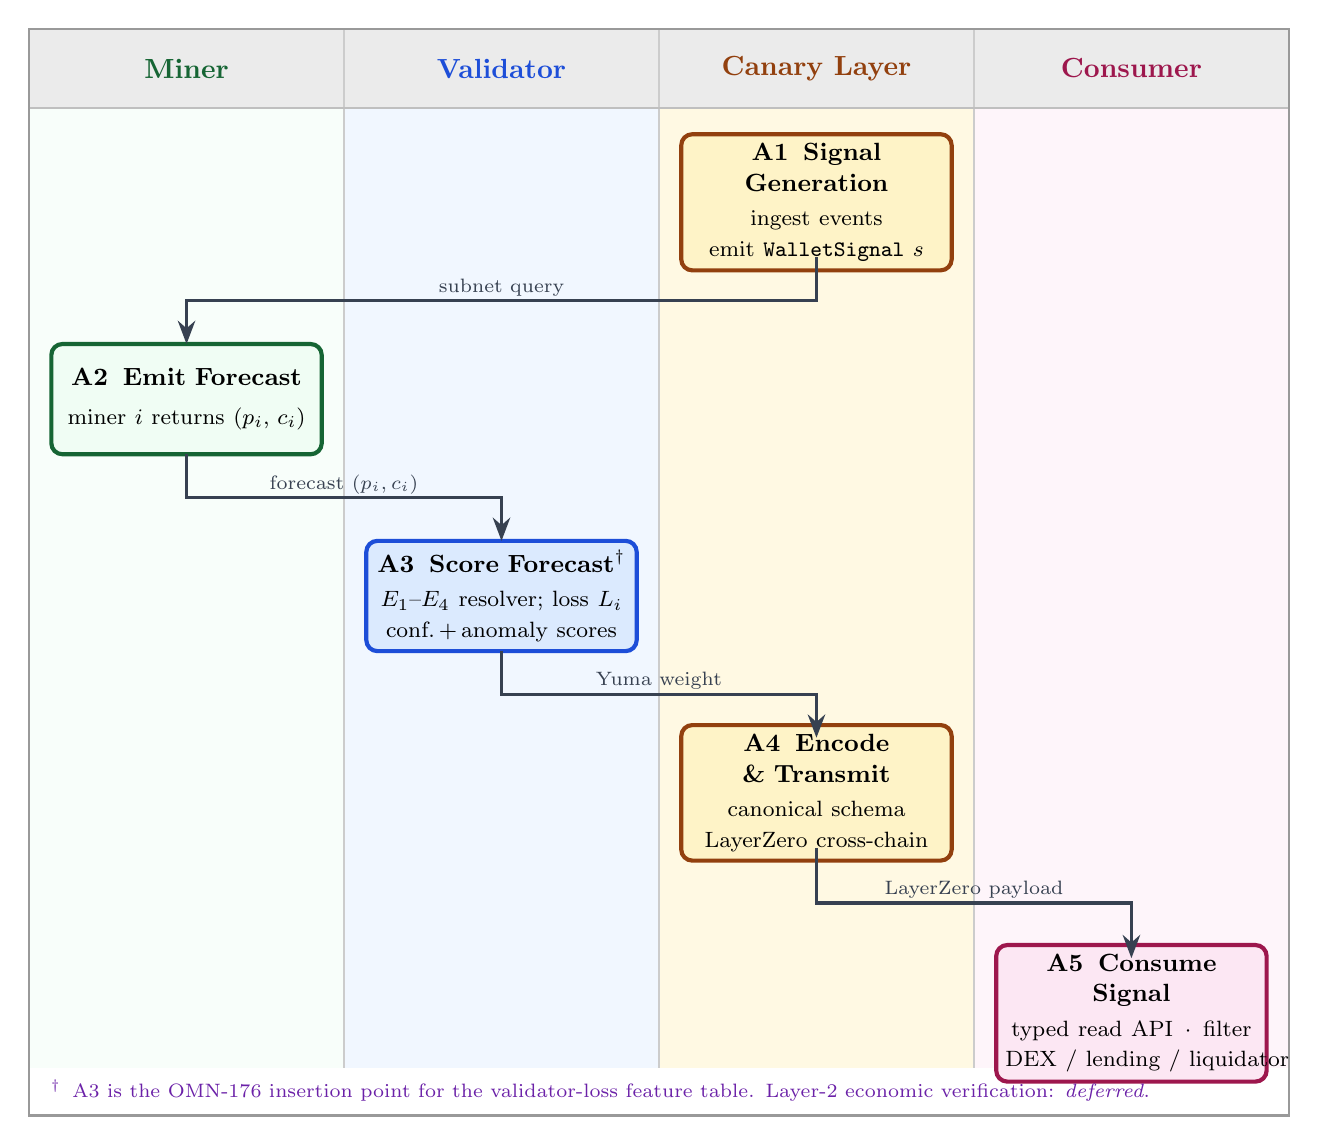
\begin{tikzpicture}[>=Stealth, thick, every node/.style={align=center}]

%%=== COORDINATE PLAN (cm) ===========================================
%%  Lanes (L→R): Miner · Validator · Canary Layer · Consumer
%%  Lane width = 4.0 each; total width = 16.0
%%  x-centres: M=2.0  V=6.0  CL=10.0  Con=14.0
%%  Lane dividers at x = 4.0, 8.0, 12.0
%%  Header row: y = 0 .. −1.0
%%  Activity y-centres: A1=−2.2  A2=−4.7  A3=−7.2  A4=−9.7  A5=−12.5
%%  Activity box: 3.4 × 1.4 cm  (half-height = 0.70)
%%  A1.south=−2.9  A2.north=−4.0  A2.south=−5.4  A3.north=−6.5
%%  A3.south=−7.9  A4.north=−9.0  A4.south=−10.4  A5.north=−11.8
%%  Lane fill area: y = 0 .. −13.2  (flush with A5.south)
%%  Footnote strip: y = −13.2 .. −13.8  (white)
%%====================================================================

%% --- Background: fills, header shade, dividers, border -------------
\begin{pgfonlayer}{background}
  %% lane fills
  \fill[minerfill!50]     (0,    0) rectangle ( 4.0,-13.2);
  \fill[validatorfill!40] (4.0,  0) rectangle ( 8.0,-13.2);
  \fill[canaryfill!50]    (8.0,  0) rectangle (12.0,-13.2);
  \fill[consumerfill!40]  (12.0, 0) rectangle (16.0,-13.2);
  %% white footnote strip
  \fill[white]            (0,-13.2) rectangle (16.0,-13.8);
  %% header tint
  \fill[black!8]          (0, 0) rectangle (16.0,-1.0);
  %% lane dividers
  \draw[black!20, line width=0.5pt]  ( 4.0, 0) -- ( 4.0,-13.2);
  \draw[black!20, line width=0.5pt]  ( 8.0, 0) -- ( 8.0,-13.2);
  \draw[black!20, line width=0.5pt]  (12.0, 0) -- (12.0,-13.2);
  \draw[black!25, line width=0.8pt]  ( 0.0,-1.0) -- (16.0,-1.0);
  %% outer border
  \draw[black!40, line width=1.0pt]  (0,0) rectangle (16.0,-13.8);
\end{pgfonlayer}

%% --- Lane headers --------------------------------------------------
\node[font=\normalsize\bfseries, text=minerstroke]
  at ( 2.0,-0.5) {Miner};
\node[font=\normalsize\bfseries, text=validatorstroke]
  at ( 6.0,-0.5) {Validator};
\node[font=\normalsize\bfseries, text=canarystroke]
  at (10.0,-0.5) {Canary Layer};
\node[font=\normalsize\bfseries, text=consumerstroke]
  at (14.0,-0.5) {Consumer};

%% --- Activity nodes ------------------------------------------------

%% A1 — Signal Generation (Canary Lane)
\node[draw=canarystroke, fill=canaryfill,
      rounded corners=4pt, line width=1.5pt,
      minimum width=3.4cm, minimum height=1.4cm,
      text width=3.2cm, font=\small]
  at (10.0,-2.2)
  {\textbf{A1\enspace Signal Generation}\\[3pt]%
   \footnotesize ingest events\\emit \texttt{WalletSignal}~$s$};

%% A2 — Emit Forecast (Miner Lane)
\node[draw=minerstroke, fill=minerfill,
      rounded corners=4pt, line width=1.5pt,
      minimum width=3.4cm, minimum height=1.4cm,
      text width=3.2cm, font=\small]
  at (2.0,-4.7)
  {\textbf{A2\enspace Emit Forecast}\\[3pt]%
   \footnotesize miner $i$ returns $(p_i,\,c_i)$};

%% A3 — Score Forecast (Validator Lane) — OMN-176 insertion hook
\node[draw=validatorstroke, fill=validatorfill,
      rounded corners=4pt, line width=1.5pt,
      minimum width=3.4cm, minimum height=1.4cm,
      text width=3.2cm, font=\small]
  at (6.0,-7.2)
  {\textbf{A3\enspace Score Forecast}$^{\dagger}$\\[3pt]%
   \footnotesize $E_1$--$E_4$ resolver; loss $L_i$\\conf.\,+\,anomaly scores};

%% A4 — Encode + LayerZero TX (Canary Lane)
\node[draw=canarystroke, fill=canaryfill,
      rounded corners=4pt, line width=1.5pt,
      minimum width=3.4cm, minimum height=1.4cm,
      text width=3.2cm, font=\small]
  at (10.0,-9.7)
  {\textbf{A4\enspace Encode \& Transmit}\\[3pt]%
   \footnotesize canonical schema\\LayerZero cross-chain};

%% A5 — Consume Signal (Consumer Lane)
\node[draw=consumerstroke, fill=consumerfill,
      rounded corners=4pt, line width=1.5pt,
      minimum width=3.4cm, minimum height=1.4cm,
      text width=3.2cm, font=\small]
  at (14.0,-12.5)
  {\textbf{A5\enspace Consume Signal}\\[3pt]%
   \footnotesize typed read API\enspace$\cdot$\enspace filter\\\mbox{DEX / lending / liquidator}};

%% --- Orthogonal staircase arrows -----------------------------------

%% A1 → A2: Canary Lane → Miner Lane (leftward)
%% A1.south=(10,−2.9); elbow y=−3.45; A2.north=(2,−4.0)
\draw[->, draw=flowcolor, line width=1.2pt]
  (10.0,-2.9) -- (10.0,-3.45) -- (2.0,-3.45) -- (2.0,-4.0);
\node[font=\scriptsize, text=flowcolor] at (6.0,-3.28) {subnet query};

%% A2 → A3: Miner Lane → Validator Lane (rightward)
%% A2.south=(2,−5.4); elbow y=−5.95; A3.north=(6,−6.5)
\draw[->, draw=flowcolor, line width=1.2pt]
  (2.0,-5.4) -- (2.0,-5.95) -- (6.0,-5.95) -- (6.0,-6.5);
\node[font=\scriptsize, text=flowcolor] at (4.0,-5.78) {forecast $(p_i,c_i)$};

%% A3 → A4: Validator Lane → Canary Lane (rightward)
%% A3.south=(6,−7.9); elbow y=−8.45; A4.north=(10,−9.0)
\draw[->, draw=flowcolor, line width=1.2pt]
  (6.0,-7.9) -- (6.0,-8.45) -- (10.0,-8.45) -- (10.0,-9.0);
\node[font=\scriptsize, text=flowcolor] at (8.0,-8.28) {Yuma weight};

%% A4 → A5: Canary Lane → Consumer Lane (rightward)
%% A4.south=(10,−10.4); elbow y=−11.1; A5.north=(14,−11.8)
\draw[->, draw=flowcolor, line width=1.2pt]
  (10.0,-10.4) -- (10.0,-11.1) -- (14.0,-11.1) -- (14.0,-11.8);
\node[font=\scriptsize, text=flowcolor] at (12.0,-10.93) {LayerZero payload};

%% --- OMN-176 footnote (white strip, below lane area) ---------------
\node[font=\scriptsize, text=hookcolor, align=left, anchor=west]
  at (0.15,-13.48)
  {$^{\dagger}$\enspace A3 is the OMN-176 insertion point for the
   validator-loss feature table.\enspace
   Layer-2 economic verification: \textit{deferred}.};

\end{tikzpicture}%
}% end \sbox

\pdfpagewidth=\dimexpr\wd\figbox + 4pt\relax
\pdfpageheight=\dimexpr\ht\figbox + \dp\figbox + 4pt\relax
\hbox to \pdfpagewidth{\hss\usebox{\figbox}\hss}
\end{document}
